\documentclass[french]{beamer}

\usepackage{hyperref}
\usepackage[utf8]{inputenc}
\usepackage[T1]{fontenc}
\usepackage{color}
\usepackage{colortbl}% http://ctan.org/pkg/xcolor
\usepackage{multirow}

\usepackage{tikz}
\usetikzlibrary{tikzmark,patterns,arrows,shapes,positioning,calc}

\hypersetup{pdfpagemode=FullScreen}


\usepackage{tcolorbox}

\usetheme{metropolis} 
\metroset{numbering=fraction}
\setbeamerfont{caption}{size=\tiny}
\setbeamertemplate{title page}{
\begin{minipage}[b][\paperheight]{\textwidth}
\vfill%
\centering
\ifx\inserttitle\@empty\else\usebeamertemplate*{title}\fi
\ifx\insertsubtitle\@empty\else\usebeamertemplate*{subtitle}\fi
\usebeamertemplate*{title separator}
\ifx\beamer@shortauthor\@empty\else\usebeamertemplate*{author}\fi
\ifx\insertinstitute\@empty\else\usebeamertemplate*{institute}\fi
\ifx\insertdate\@empty\else\usebeamertemplate*{date}\fi
\vfill
\vspace*{1mm}
\end{minipage}
}
\setbeamertemplate{title}{
%  \raggedright%
\vspace*{2em}
\linespread{.8}%
\inserttitle%
\par%
\vspace*{0.5em}
}
\setbeamertemplate{subtitle}{
%  \raggedright%
\insertsubtitle%
\par%
\vspace*{0.1em}
}

\setlength\abovecaptionskip{1pt}
\setlength\belowcaptionskip{3pt}
\setlength{\textfloatsep}{5pt}

\usepackage{array}
\newcolumntype{L}[1]{>{\raggedright\let\newline\\\arraybackslash\hspace{0pt}}m{#1}}
\newcolumntype{C}[1]{>{\centering\let\newline\\\arraybackslash\hspace{0pt}}m{#1}}


\title{Multilevel models in epidemiology}
\subtitle{{\em An application to chikungunya and Zika epidemics}}
\author{Advanced statistical methods for physicists}
\institute{ Julien Riou \\
	\textit{Institute of Social and Preventive Medicine  \\ 	University of Bern }
\vspace{1.5em}
}
\date{Bern, 31 May 2019 }

\begin{document}

\tikzstyle{every picture}+=[remember picture]
\everymath{\displaystyle}

\frame[noframenumbering]{\titlepage}

\frame{
	\frametitle{Themes}
	
	Provide a real-world example of model development in relation to a scientific question:
	\begin{itemize}
		\item Mechanistic model (data-generating processes)
		\item Multilevel structure in relation to data structure
		\item Partial pooling of information
		
	\end{itemize}
}

\section{The global invasion of \textit{Aedes} mosquitoes}


\frame{
	\frametitle{{\em Aedes} mosquitoes (i)}
	% Plus de 250 espèces
	% abdomen long et étroits, motifs noirs et blancs
	% cycle de vie en 4 stades: oeuf, larve, pupe, adulte
	\begin{figure}[h]
		\centering
		\includegraphics[width=9cm]{Figures/mosquitolifecyle_ext3.png}
		\vspace{-1em}
		\caption{Life cycle of {\em Aedes} mosquitoes.}
	\end{figure}
	\begin{itemize}
		\vspace{-.5em}
		\item[-] Blood meal necessary to egg maturation
		
		\item[-] Biting behaviour: \alert{gonotrophic cycle}
		
		\item[-] Transmission through saliva: specific vectorial competence %virus adapté à l'espèce de moustique
	\end{itemize}
}

\frame{
	\frametitle{{\em Aedes} mosquitoes (ii)}
	
	Two species are important to human health:
	
	\begin{itemize}
		\item[-] \alert{\em Aedes aegypti} (tropical and subtropical areas)
		
		\vspace{.5em}
		\item[-] \alert{\em Aedes albopictus} (subtropical et temperate areas)
	\end{itemize}
	
	\begin{figure}[h]
		\centering
		\includegraphics[width=8cm]{Figures/aegyptialbopictusCDC.jpg}
		\caption{Female adult specimens of {\em Aedes aegypti} (left) and {\em Aedes albopictus} (right).}
	\end{figure}
	\vfill
}


\frame{
	\frametitle{The domestication of {\em Aedes aegypti}}
	
	\begin{figure}[h]
		\centering
		\includegraphics[width=10cm]{Figures/repartitionaedesaegypti2.png}
		\caption{World distribution of {\em Aedes aegypti} $^1$.}
	\end{figure}
	\begin{itemize}
		\vspace{-.5em}
		\item[-] Originally from Africa, extension from the 15th century % traite des esclaves: principal lien entre Afrique et Amériques	
		\vspace{.5em}
		\item[-] \alert{Urban} and \alert{domestic} species: adapted to human settlements$^2$ % piqûre préférentielle des humains, oviposition dans des récipients artificiels: ne dépend plus de la pluie
		
	\end{itemize}
	\vfill\vspace{2em}
	\setcounter{footnote}{1} \footnotetext{
		{\tiny Kraemer et al., \textit{eLife} (2015) ; $^2$ Powell et Tabachnick, \textit{Memorias do Instituto Oswaldo Cruz} (2013)}
	}
}

\frame{
	\frametitle{The invasion of {\em Aedes albopictus}}
	
	\begin{figure}[h]
		\centering
		\includegraphics[width=10cm]{Figures/repartitionaedesalbopictus2.png}
		\caption{World distribution of {\em Aedes albopictus} $^1$.}
	\end{figure}
	\begin{itemize}
		\vspace{-.5em}
		\item[-] Originally from Asia, extension from the 20th century$^2$ % trafic international de pneus usagers
		\vspace{.5em}
		\item[-] \alert{Invasive} species: plasticity, competitive advantages$^3$ % vis à vis d'autres espèces lorsqu'il est introduit dans un milieu
	\end{itemize}
	\vfill\vspace{2em}
	\setcounter{footnote}{1} \footnotetext{
		\tiny{Kraemer et al., \textit{eLife} (2015) ; $^2$Reiter, \textit{Journal of the American Mosquito Control Assoc.} (1998) ; $^3$Paupy et al., \textit{Microbes and Infection} (2009)}
	}
}


\frame{
	\frametitle{Disease emergences}
	
	\scalebox{.9}{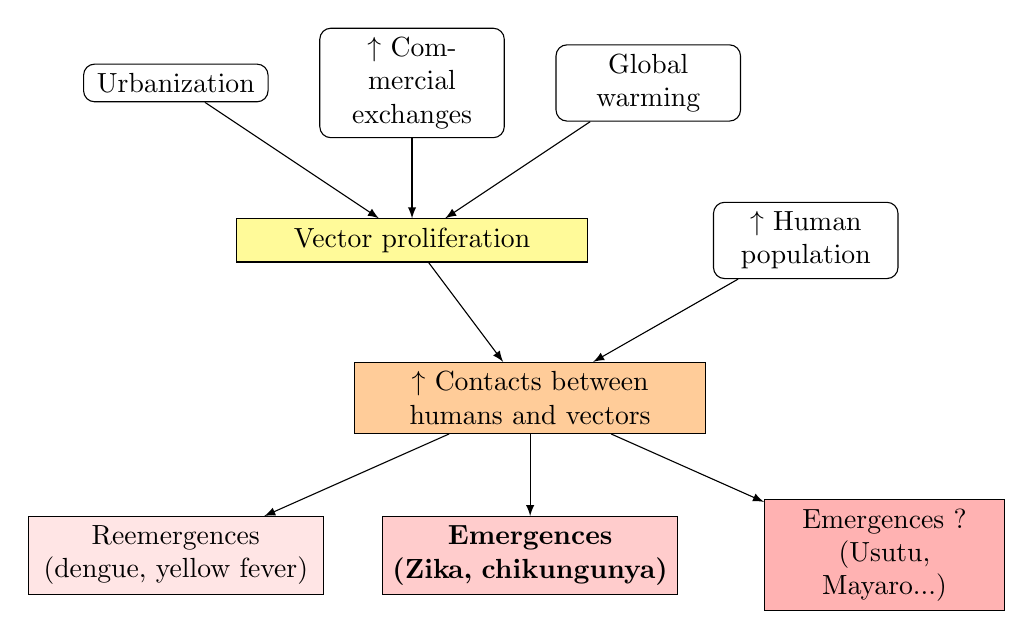
\begin{tikzpicture}
		\node[rounded corners,draw,text width=6em,align=center] (a) at (0,1) {Urbanization};
		\node[rounded corners,draw,text width=6em,align=center] (b) at (3,1) {$\uparrow$ Commercial exchanges};
		\node[rounded corners,draw,text width=6em,align=center] (d) at (6,1) {Global warming};	
		
		\node[draw,text width=12em,align=center,fill=yellow!40] (e) at (3,-1) {Vector proliferation};	
		
		\node[rounded corners,draw,text width=6em,align=center] (c) at (8,-1) {$\uparrow$ Human population};	
		
		\node[draw,text width=12em,align=center,fill=orange!40] (e2) at (4.5,-3) {$\uparrow$ Contacts between humans and vectors};	
		
		\node[draw,text width=10em,align=center,fill=red!10] (f) at (0,-5) {Reemergences \\ (dengue, yellow fever)};
		\node[draw,text width=10em,align=center,fill=red!20] (g) at (4.5,-5) {Emergences \\ (Zika, chikungunya)};
		\node[draw,text width=8em,align=center,fill=red!30] (h) at (9,-5) {Emergences ? \\ (Usutu, Mayaro...)};
		
		\draw[->,>=latex] (a) -- (e);
		\draw[->,>=latex] (b) -- (e);
		\draw[->,>=latex] (c) -- (e2);
		\draw[->,>=latex] (d) -- (e);
		\draw[->,>=latex] (e) -- (e2);
		
		\draw[->,>=latex] (e2) -- (f);
		\draw[->,>=latex] (e2) -- (g);
		\draw[->,>=latex] (e2) -- (h);
		\pause
		\node[draw,text width=10em,align=center,fill=red!20] (g) at (4.5,-5) {\textbf{Emergences \\ (Zika, chikungunya)}};
		\end{tikzpicture}}
}

\frame{
	\frametitle{World propagation of chikungunya (CHIKV)}
	% isolé en Tanzanie en 1953
	% 2005: émergence de la souche IOL (indian ocean lineage), épidémie à la Réunion
	% extension vers l'Asie du sud-est, importations et transmission locale en Europe
	% 2013-2016: épidémie aux Antilles françaises, puis dans les zones tropicales d'Amérique, puis vers le Pacifique
	\vspace{1em}
	\begin{figure}[h]
		\centering
		\includegraphics[width=\linewidth]{Figures/weaver_chik2.png}
		\caption{Origin and extension of the chikungunya virus and his vectors$^1$.}
	\end{figure}
	\vfill\vspace{2em}
	\setcounter{footnote}{1} \footnotetext{
		\tiny{Weaver et al., \textit{New England Journal of Medicine} (2015)}
}}

\frame{
	\frametitle{World propagation of Zika (ZIKV)}
	% forêt Zika, en Ouganda 1947
	% retrouvé sporadiquement en Afrique subsaharienne, en Egypte, en Asie du sud-est
	% épidémie à Yap en 2007
	% épidémies en Polynésie française en 2013, puis au Brésil en 2015
	\vspace{1em}
	\begin{figure}[h]
		\centering
		\includegraphics[width=\linewidth]{Figures/zikaspread.png}
		\caption{Origin and extension of the Zika virus$^1$.}
	\end{figure}
	\vfill\vspace{2em}
	\setcounter{footnote}{1} \footnotetext{
		\tiny{Gatherer et Kohl, \textit{Journal of General Virology} (2016)}
}}


\section{Comparing Zika and chikungunya epidemics}

\frame{
	\frametitle{Strategy}
	Successive waves of chikungunya and Zika epidemics:
	\begin{itemize}
		\item each circulating for the first time
		\item in the same areas
		\item within a short timespan
	\end{itemize}

	$\Rightarrow$ \alert{Comparison} of epidemics of different viruses: 
	\begin{itemize}
	\item in the same populations (immunologically naive)
	\item in the same environments (vectors)
	\item observed by the same surveillance systems
\end{itemize}

}

\frame{
	\frametitle{Data}
	Time-series of \alert{incidence data} for 18 outbreaks of ZIKV and CHIKV:
	\begin{itemize}
		\item weekly number of reported cases CHIKV or ZIKV
		\item between 2013 and 2016
		\item in 9 islands with similar surveillance systems

	\end{itemize}
	
	\begin{figure}[h]
		\centering
		\includegraphics[width=\linewidth]{Figures/screen_data.png}
	\end{figure}

	\url{https://github.com/jriou/multilevel_models_epi}
}


\frame{
	\frametitle{Data}

	\begin{figure}[h]
		\centering
		\includegraphics[width=9cm]{Figures/Fig1_revised2.pdf}
		\setlength\abovecaptionskip{-2mm}
		\caption{Profiles of CHIKV (red) and ZIKV (blue) incidence in nine territories during 2013--2016.}
	\end{figure}
}

\frame{
	\frametitle{Data-generating processes: observation}
	How is the number of reported cases on week $t$ (\alert{$O_t$}) generated?
	\pause
	\begin{itemize}
		\item true number of infections by CHIKV or ZIKV ($I_t$)
		\item with symptoms (70\% for CHIKV, 20-30\% for ZIKV)
		\item sufficient to lead to a consultation with a physician
		\item recognized by the physician
		\item reported by the physician to the surveillance authorities
	\end{itemize}
	\pause
	
	At the observation level:
		$$ 	O_t \sim \text{Binom}(I_t,\alert{\rho}) $$

	$\Rightarrow$ \alert{Parameter $\rho$}:  probability of reporting 
}

\frame{
	\frametitle{Data-generating processes: transmission}
	How it the true number of infections (\alert{$I_t$}) generated?
	\pause
	\begin{itemize}
		\item (if we ignore importations)
		\item all new cases can be linked back to cases in the last few weeks
		\item with a delay corresponding to the actions of the vector
	\end{itemize}
	\pause
	
	At the transmission level:
		$$I_t \sim \text{Binom}\left(S_t,\alert{\beta} 
		\fcolorbox{black!80}{blue!30}{$\frac{1}{N}\sum^5_{n=1}w_{t,n}I_{t-n}$}\right)$$
	
	$\Rightarrow$ \alert{Parameter $\beta$}: number of secondary cases by primary case ($\mathcal{R}_0$)

	$\Rightarrow$ \textcolor{blue!30}{Exposure}: depends on the serial interval $w_t$
}



\frame{
	\frametitle{The serial interval}

	\vspace{1em}
	\metroset{block=fill}
	\begin{alertblock}{Definition}
		\underline{Serial interval}: the time between the disease onset of a primary case and one of its secondary cases\textsuperscript{1} 
	\end{alertblock}
	
	Reconstruction using the full \alert{transmission cycle}
	\vspace{-2mm}
	\begin{figure}[h]
		\centering
		\only<1>{\begin{tikzpicture}
		\node[anchor=south west,inner sep=0] at (0,0) {\includegraphics[width=7cm]{Figures/serialinterval0.png}};		
		\end{tikzpicture}}\only<2>{\begin{tikzpicture}
		\node[anchor=south west,inner sep=0] at (0,0) {\includegraphics[width=7cm]{Figures/serialinterval0.png}};
		\draw[->,orange,thick] (2.4,1.4) -- (2.4,2.55) ;		
		\draw[->,orange,thick] (5.1,1.4) -- (5.1,1.6) ;		
		\draw[orange,dotted] (2.4,1.4) -- (5.1,1.4) ;		
		\end{tikzpicture}}\only<3>{\begin{tikzpicture}
		\node[anchor=south west,inner sep=0] at (0,0) {\includegraphics[width=7cm]{Figures/serialinterval4.png}};
		\draw[->,orange,thick] (2.4,1.4) -- (2.4,2.55) ;		
		\draw[->,orange,thick] (5.1,1.4) -- (5.1,1.6) ;		
		\draw[orange,dotted] (2.4,1.4) -- (5.1,1.4) ;		
		\end{tikzpicture}}
		\caption{Framework for calculating the distribution of the serial interval\textsuperscript{2}.}
	\end{figure} 
		\setcounter{footnote}{1} \footnotetext{
			\tiny{Svensson et al, \textit{Math. biosciences} (2007)};\textsuperscript{2}Boëlle et al, \textit{Vector-borne and zoonotic diseases} (2007)
		}
}


\frame{
	\frametitle{The serial interval}
	Using \alert{published data} on each stage (including dependence to local temperature $T$) we obtain:
	\begin{equation*}
		T_{SI} = -T_V + T_B + T_M(T) + T_I
	\end{equation*}
	\begin{figure}[h]
		\centering
		\includegraphics[width=8cm]{Figures/Fig2B.pdf}
		\caption{Distribution of the serial interval for CHIKV (red) and ZIKV (blue) according to temperature.}
	\end{figure} 
}


\frame{
	\frametitle{One disease, one island: model}

	Let $O_t$ be the observed incidence in one epidemic on week $t$:
	\begin{itemize}
    \item[-] at the \alert{observation} level: 
		\[O_t \sim \text{Binom}(I_t,\tikzmark{a}\fcolorbox{black!80}{red!30}{$\rho$})\]
		\begin{tikzpicture}[draw=black!80,remember picture,overlay]
			\draw[->] ([xshift=0.5em+2\fboxrule,yshift=1ex+\fboxsep-\fboxrule]pic cs:a) |- ++(+15:60pt) coordinate (A);
			\node[style={rounded corners,draw=black!80,fill=red!20,inner sep = 4pt},xshift=0ex,yshift=0pt,draw] at (A) {Reporting rate};
		\end{tikzpicture}
	\pause
    \item[-] at the \alert{transmission} level: \\
		\[I_t \sim \text{Binom}\left(
					\tikzmark{b}\fcolorbox{black!80}{brown!30}{$S_t$}
					,
					\tikzmark{c}\fcolorbox{black!80}{green!30}{$\beta$}
					\tikzmark{d}\fcolorbox{black!80}{blue!30}{$\frac{1}{N}\sum^5_{n=1}w_{t,n}I_{t-n}$}
					\right)\]
		\begin{tikzpicture}[draw=black!80,remember picture,overlay]
			\draw[->] ([xshift=.8em,yshift=1em]pic cs:b) |- ++(-15:-60pt) coordinate (B);
			\node[style={rounded corners,draw=black!80,fill=brown!20,inner sep = 4pt},xshift=0ex,yshift=0pt,draw] at (B) {Susceptibles};
		\end{tikzpicture}
		\begin{tikzpicture}[draw=black!80,remember picture,overlay]
			\draw[->] ([xshift=.8em,yshift=1em]pic cs:c) |- ++(+40:60pt) coordinate (C);
			\node[style={rounded corners,draw=black!80,fill=green!20,inner sep = 4pt},xshift=0ex,yshift=0pt,draw] at (C) {Transmission};
		\end{tikzpicture}
		\begin{tikzpicture}[draw=black!80,remember picture,overlay]
			\draw[->] ([xshift=3em,yshift=2.1em]pic cs:d) |- ++(+8:70pt) coordinate (D);
			\node[style={rounded corners,draw=black!80,fill=blue!20,inner sep = 4pt},xshift=0ex,yshift=0pt,draw] at (D) {Exposure};
		\end{tikzpicture}
	\pause
	 \item[-] both levels simplify into:
		\[	O_t \sim \text{Neg-Binom}\left(S_t \frac{\beta}{N} \sum^5_{n=1}w_{t,n}\frac{O_{t-n}}{\rho}, 
				\tikzmark{e}\fcolorbox{black!80}{pink!30}{$\phi$}\right) \]
		\begin{tikzpicture}[draw=black!80,remember picture,overlay]
			\draw[->] ([xshift=.6em,yshift=1em]pic cs:e) |- ++(-20:-60pt) coordinate (E);
			\node[style={rounded corners,draw=black!80,fill=pink!20,inner sep = 4pt},xshift=0ex,yshift=0pt,draw] at (E) {Overdispersion};
		\end{tikzpicture}

	\end{itemize}

}


\frame{
	\frametitle{One disease, one island: implementation in Stan}
	
	In a separate \texttt{.stan} file:
	\begin{itemize}
		\item Data block:
		\vspace{1em}
		
		\includegraphics[width=8cm]{Figures/stan1.png}
		
		\pause\item Parameters block:
		\vspace{1em}
		
		\includegraphics[width=8cm]{Figures/stan2.png}
	\end{itemize}
	
}

\frame{
	\frametitle{One disease, one island: implementation in Stan}
	
	\begin{itemize}
		\item Transformed parameters block:
		\vspace{1em}
		
		\includegraphics[width=8cm]{Figures/stan3.png}
		
		{\tiny$$\text{NB:} ~~ S_t \frac{\beta}{N} \sum^5_{n=1}w_{t,n}\frac{O_{t-n}}{\rho} = \left(1 - \frac{\sum_t O_t}{\rho N}\right)\beta O^*_t$$}
		
		\pause\item Model block:
		\vspace{1em}
		
		\includegraphics[width=8cm]{Figures/stan4.png}
	\end{itemize}
}


\frame{
	\frametitle{One disease, one island: implementation in Stan}
	
	Control \texttt{Stan} from \texttt{R} with \texttt{library(rstan)}:

		\includegraphics[width=8cm]{Figures/stan5.png}
	\pause
	
	Results: \alert{posterior distributions} of $\beta$, $\rho$ and $\phi$
	
	\includegraphics[width=8cm]{Figures/stan6.png}
	
}


\frame{
	\frametitle{One disease, one island: implementation in Stan}
	

	\begin{figure}
		\centering
			\includegraphics[width=8cm]{Figures/fit.png}
			\caption{Model fit for the epidemic of Zika virus in Guadeloupe.}
	\end{figure}

}

\frame{
	\frametitle{Now for 9 islands}
	Degrees of pooling:
	\begin{itemize}
		\item independent $\beta_i$ and $\rho_i$ for each island: \alert{no pooling} 
		
		\pause\hspace{1em}\item the same $\beta$ and $\rho$ for all islands: \alert{complete pooling}
				 
		\pause\hspace{1em}\item \textit{correlated} $\beta_i$ and $\rho_i$ for each island: \alert{partial pooling}
			\begin{itemize}
				\item[=] multilevel or hierarchical
			\end{itemize}
	\end{itemize}
}

\frame{
	\frametitle{Now for 9 islands}
	For the epidemic in island $i$, we have:
	\begin{itemize}
		\item a transmission parameter $\beta_i$ which depends on \alert{hyperparameters} $\mu_{\beta}$ and $\sigma_{\beta}$:
		
				$$\ln \beta_{i,j=0} \sim \mathcal{N}(\mu_{\beta},\sigma_{\beta}^2) $$
		
		\pause\item a reporting parameter $\rho_i$ which depends on \alert{hyperparameters} $\mu_{\rho}$ and $\sigma_{\rho}$:
		
		$$\ln\frac{\rho_{i,j=0}}{1-\rho_{i,j=0}} \sim \mathcal{N}(\mu_{\rho},\sigma_{\rho}^2) $$
	\end{itemize}

	\pause \vspace{2em}
	\alert{$\Rightarrow$ We now also estimate $\mu_{\beta}$, $\mu_{\rho}$, $\sigma_{\beta}$ and $\sigma_{\rho}$ }
	
}

\frame{
	\frametitle{Now for 9 islands and 2 diseases}
	
	We now model together the epidemics of ZIKV ($j=1$) and CHIKV ($j=0$) assuming \alert{proportionality}:
	\begin{itemize}
		\item on the transmission parameters of ZIKV and CHIKV:
		$$\beta_{i,j=1} = \eta \times \beta_{i,j=0}$$
		\item on the reporting parameters of ZIKV and CHIKV (on the logit scale):
		$$ \frac{\rho_{i,j=1}}{1-\rho_{i,j=1}} = \omega \times  \frac{\rho_{i,j=0}}{1-\rho_{i,j=0}}$$
	\end{itemize}
	
		\pause \vspace{2em}
	\alert{$\Rightarrow$ We now also estimate $\eta$ and $\omega$}
	
}



\frame{
	\frametitle{Now for 9 islands and 2 diseases}
	The \alert{model fit} is acceptable for CHIKV:
	\begin{figure}[h]
		\centering
		\includegraphics[width=9cm]{Figures/Fig3_revised_CHIKV.pdf}
		\caption{Model fit for the CHIKV epidemics.}
	\end{figure} 
}



\frame{
	\frametitle{Now for 9 islands and 2 diseases}
	And for ZIKV:
	\begin{figure}[h]
		\centering
			\includegraphics[width=9cm]{Figures/Fig3_revised_ZIKV.pdf}
		\caption{Model fit for the ZIKV epidemics.}
	\end{figure} 
}

\frame{
	\frametitle{Now for 9 islands and 2 diseases}
	The main results are:
	\begin{itemize}
		\item[-] a \alert{similar transmissibility} of CHIKV and ZIKV within an area
			\begin{itemize}
					\item $\eta|\text{data}=1.04 \;[0.97-1.13]$
			\end{itemize}
		\vspace{.5em}
		\item[-] a \alert{lower reporting rate for ZIKV}
			\begin{itemize}
					\item $\omega|\text{data} = 0.37\;[0.34-0.40]$
			\end{itemize}
		\vspace{1em}
		\begin{figure}[h]
			\centering
			\includegraphics[width=4cm]{Figures/res1.pdf}\hspace{2em}
			\includegraphics[width=4cm]{Figures/res2.pdf}
		\vspace{-2mm}
			\caption{Posterior estimates of $\mu_{\beta}$ and $\mu_{\rho}$ for CHIKV and ZIKV.}
		\end{figure} 

	\end{itemize}
}

\frame{
	\frametitle{Now for 9 islands and 2 diseases}
	We also find \alert{heterogeneity} between areas:
	\begin{itemize}
		\item[-] $\sigma_{\beta}^2|\text{data} > 0$, lower $\beta$ in the French West Indies
		\item[-] $\sigma_{\rho}^2|\text{data} > 0$, higher $\rho$ in small islands and in Martinique
\vspace{1em}
\end{itemize}
	\begin{figure}[h]
		\centering
			\includegraphics[width=5cm]{Figures/het1.pdf}\hspace{1em}
			\includegraphics[width=5cm]{Figures/het2.pdf}
		\vspace{-2mm}
		\caption{Island-specific posterior estimates of $\beta$ and $\rho$ for CHIKV (red) and ZIKV (blue).}
	\end{figure} 
}



\frame{
	\frametitle{Conclusion}
	Remember about:
	\begin{itemize}
		\item Data-generating mechanisms
		\vspace{1em}
		
		\item Plot model predictions (fit)
		\vspace{1em}
		
		\item Multi-level structure following data structure (partial pooling)
	\end{itemize}

}



\end{document}
